\documentclass[12pt,a4paper]{article}
\usepackage[utf8]{vietnam}
\usepackage{fontspec}
\setmainfont{Times New Roman}
\usepackage{indentfirst}
\usepackage{hyperref}
\usepackage{tikz}
\usepackage[left=2.64cm,right=2.54cm,top=2cm,bottom=2cm]{geometry}
\usepackage{geometry}
\usepackage{array}
\usepackage{color}
\usepackage{wallpaper}
\setcounter{page}{2}
\makeatletter
\definecolor{dkgreen}{rgb}{0,0.6,0}
\definecolor{gray}{rgb}{0.5,0.5,0.5}
\definecolor{mauve}{rgb}{0.58,0,0.82}
\usepackage{listings}
\pagenumbering{arabic}
\usepackage{fancyhdr}
\usepackage{lastpage}
\usepackage{minitoc}
\pagestyle{fancy}
\fancyhf{}
\rhead{21127511 Nguyễn Quốc Huy}
\lhead{Vật lý đại cương}
\rfoot{Trang \thepage \hspace{1pt}  \pageref{LastPage}}
\usepackage{multicol}
\setlength{\columnsep}{1cm}
\begin{document}
\thispagestyle{empty}
\begin{LARGE}
    \begin{center}{\underline{\color{red}{\bf NATIONAL UNIVERSITY OF HO CHI MINH CITY}}}
    \end{center}
\end{LARGE}
\vspace*{1cm}
\begin{center}{\Huge \color{green}\textbf{KHOA CÔNG NGHỆ THÔNG TIN}}
\end{center}
\ThisCenterWallPaper{1}{New_KHTN.jpg}
\vspace*{15cm}
\begin{center}{\Huge \color{cyan}\textbf{Nguyễn Quốc Huy - 21127511}}
\end{center}
\vspace*{1cm}
\begin{center}
    {\Huge \color{cyan}\textbf{{LỚP 21CLC02 - VẬT LÝ ĐẠI CƯƠNG}}}
\end{center}
\newpage
\let\cleardoublepage\clearpage

\tableofcontents

\newpage
\section{\textbf{\color{red}CHƯƠNG 3: CÁC ĐỊNH LUẬT BẢO TOÀN}}
\Large \subsection{\color{blue}\textbf{BÀI 1} }

\vspace*{1cm}
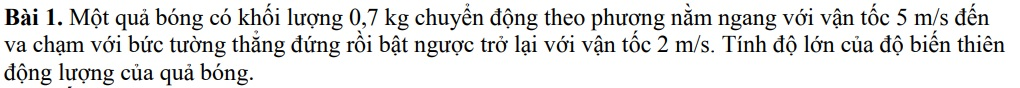
\includegraphics[scale=0.80]{No1.jpg}

\vspace*{1cm}
Độ biến thiên động lượng : 

$\Delta p = P_2 - P_1 = mv_2 - mv_1 = 0,7.5 - 0,7.(-2) = 4,9$ (kg.m/s)
\Large \subsection{\color{blue}\textbf{BÀI 2} }

\vspace*{1cm}
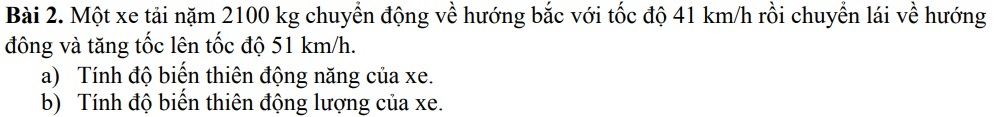
\includegraphics[scale=0.80]{No2.jpg}

\vspace*{1cm}
Độ biến thiên động năng : 

$\Delta K = K_2 - K_1 = \frac{mv_2^2}{2} - \frac{mv_1^2}{2} =  \frac{m(v_2^2 - v_1^2)}{2}$

\vspace*{1cm}
$\to\Delta K = \frac{2100(14,17^2 - 11,14^2)}{2} \approx 7,5.10^4 (J)$

\vspace*{1cm}
Độ biến thiên động lượng:

\vspace*{1cm}
$\Delta \vec{p} = \vec{P_2} - \vec{P_1}$ nhưng hướng Bắc $\perp$ hướng Đông

\vspace*{1cm}
$ \Rightarrow p = \sqrt{P_2^2 + P_1^2} = \sqrt{(mv_2)^2 + (mv_1)^2} $

\vspace*{1cm}
$ \Leftrightarrow \sqrt{(2100.14,17)^2 + (2100.11,4)^2} \approx 3,8.10^4 (kg.m/s)$

\Large \subsection{\color{blue}\textbf{BÀI 3} }

\vspace*{1cm}
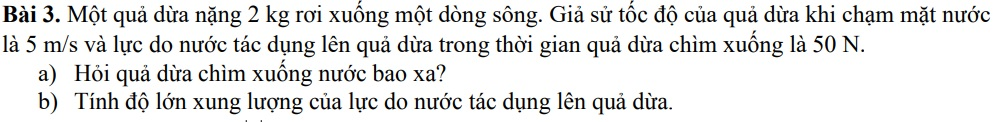
\includegraphics[scale=0.80]{No3.jpg}

\vspace*{1cm}
Ta có : $\Delta K + \Delta U = A$

\vspace*{1cm}
$\Leftrightarrow \frac{mv^2}{2} + mgS = F_n.S$
$\Leftrightarrow \frac{2.5^2}{2} - 9,8.2.S = 50.S $

\vspace*{1cm}
(Chọn gốc tọa độ khi vật dừng ở nước)

\vspace*{1cm}
$\Leftrightarrow S = 0,82 (m)$

\vspace*{1cm}
Xung lượng : $|\Delta \vec{p} | = \vec{P_2} - \vec{P_1} $

\vspace*{1cm}
$\Rightarrow| mv_2 - mv_1| = |-mv_1| = |-2.5| = 10 (m/s)$

\Large \subsection{\color{blue}\textbf{BÀI 4} }

\vspace*{1cm}
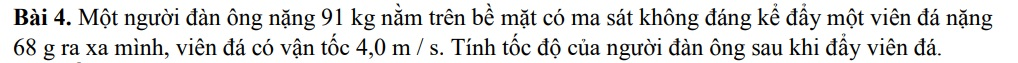
\includegraphics[scale=0.80]{No4.jpg}

\vspace*{1cm}
Ta xét định luật bảo toàn động lượng : 

\vspace*{1cm}
$\vec{p_1} =\vec{p_2} \Leftrightarrow m_1v_1 = m_2v_2 \Leftrightarrow 91.v_1 = 0,068.4$

\vspace*{1cm}
$\rightarrow v_1 = \frac{0,068.4}{91} \approx 3.10^{-3} (m/s)$

\vspace*{1cm}
\Large \subsection{\color{blue}\textbf{BÀI 7} }
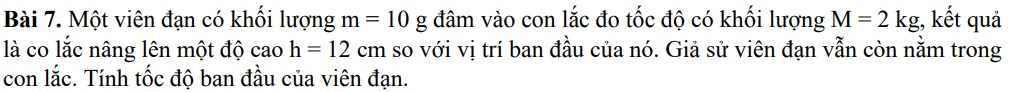
\includegraphics[scale=0.80]{No7.jpg}

\vspace*{1cm}
Gọi V là vận tốc của hệ sau va chạm ( hệ gồm viên đạn và con lắc).

Theo định luật bảo toàn động lượng:

\vspace*{1cm}
$mv + 0 = (m + M)V \Rightarrow V = \frac{mv}{m + M} $ (1)

\vspace*{1cm}
Áp dụng định luật bảo toàn cơ năng: 

\vspace*{1cm}
$ \frac{(m + M)V^2}{2} = (m + M).g.h \Rightarrow V = \sqrt{2gh}$ (2)

\vspace*{1cm}
Từ (1) và (2) $\Leftrightarrow V = \frac{mv}{m + M} = \sqrt{2gh}$

\vspace*{1cm}
$\Leftrightarrow v = \frac{m + M}{m}. \sqrt{2gh} = \frac{0,01 + 2}{0,01} . \sqrt{2.10.0,12} \approx 3,1 . 10^2 (m/s)$

\end{document}